\chapter{矩阵及其运算}\label{ch:2.1}

本节课将介绍矩阵的相关理论.考虑到大部分同学之前没有接触过矩阵,我们会通过一些实际的例子来引入矩阵的概念.矩阵最初的定义仅仅是为了简化一些式子的表示,不是很复杂的概念.所以,虽然大家没有接触过,但是矩阵的学习不是很困难,大家理解之后会发现矩阵的原理其实很简单.

本节课的主要内容包括:
\begin{enumerate}
	\item 矩阵的概念;
	\item 矩阵的运算;
	\item 矩阵的转置;
	\item 矩阵的行列式.
\end{enumerate}

\section{矩阵的概念}
在给出矩阵的定义之前,我们先来看几个平面上几种变化的例子.
\begin{example}
	在直角坐标系$Oxy$内,将每个点绕原点$O$按逆时针方向旋转$\theta$的变换称为\textbf{旋转变换}.我们首先写出这个旋转变换的表达式.

	点$M$的新坐标$\left(x',y'\right)$和旧坐标$\left(x,y\right)$之间的关系为:
	\begin{equation}\label{tran1}
		\left\{\begin{matrix}
			x=x'\cos\theta-y'\sin\theta , \\
			y={x}'\sin\theta+y'\cos\theta.
		\end{matrix}\right.
	\end{equation}

	由于\eqref{tran1}式的右端式子中$x',y'$的系数唯一确定,我们可以把这些系数按原来的顺序写出来,并在两端分别加一个括号,得到一个正方形数表.
	$\begin{bmatrix}
			\cos\theta & -\sin\theta \\
			\sin\theta & \cos\theta
		\end{bmatrix}$	.
	可以发现,这个正方形数表是由旋转角是$\theta$的旋转变换唯一确定的;反之,旋转角是$\theta$的旋转变换也可以由这个正方形数表唯一确定.所以,这个正方形数表就唯一刻画了旋转角是$\theta$的旋转变换.
\end{example}

事实上,在平面直角坐标系$Oxy$内,很多几何变换都有以下形式:
\begin{equation}\label{tran2}
	\left\{\begin{matrix}
		x=ax'+by' , \\
		y=cx'+dy'.
	\end{matrix}\right.
\end{equation}

类似地,我们引入正方形数表
$\begin{bmatrix}
		a & b \\
		c & d
	\end{bmatrix}$	,
那么几何变换\eqref{tran2}就可以由
$\begin{bmatrix}
		a & b \\
		c & d
	\end{bmatrix}$
唯一确定,
$\begin{bmatrix}
		a & b \\
		c & d
	\end{bmatrix}$
也可以由几何变换\eqref{tran2}唯一确定.

这就启发我们来研究形如以上两个数表的性质,这将对一些数学表示和研究带来便利.我们把这样的一个数表称为\textbf{矩阵}.

\begin{definition}[\textbf{矩阵}]
	由$m\times n $个数$a_{ij}\left(i=1,2,\cdots,m; j=1,2,\cdots,n\right)$排成的$m$行,$n$列的矩阵数表
	\[
		\begin{bmatrix}
			a_{11} & a_{12} & \cdots & a_{1n} \\
			a_{21} & a_{22} & \cdots & a_{2n} \\
			\vdots & \vdots & \ddots & \vdots \\
			a_{m1} & a_{m2} & \cdots & a_{mn}
		\end{bmatrix}
	\]
	称为一个$m\times n$矩阵.其中$a_{ij}$称为该矩阵的第$i$行第$j$列元素,简称该矩阵的$\left(i,j\right)$元素$i$与$j$分别称为元素$a_{ij}$的行标与列标.
\end{definition}

我们也可以把这样一个矩阵简记为$\mathbf{A}=\left(a_{ij}\right)_{m\times n}$或$\mathbf{A}_{m\times n}.$

元素是实(复)数的矩阵称为\textbf{实(复)矩阵}.

当$m=n$时,矩阵$\mathbf{A}=\left(a_{ij}\right)_{m\times n}$称为\textbf{$n$阶方阵}或\textbf{$n$阶矩阵}.对于$\mathbf{A}=\left(a_{ij}\right)_{m\times n}$,元素$a_{11},a_{22},\cdots,a_{nn}$所在的对角线称为$\mathbf{A}$的\textbf{主对角线}.

下面介绍几种特殊矩阵:
\begin{enumerate}
	\item \textbf{零矩阵}:所有元素都是零的$m\times n$矩阵称为零矩阵,记为$\mathbf{O}_{m\times n},$即
	    \[
		    \begin{bmatrix}
			    0      & 0      & \cdots & 0      \\
			    0      & 0      & \cdots & 0      \\
			    \vdots & \vdots & \ddots & \vdots \\
			    0      & 0      & \cdots & 0
		    \end{bmatrix}
	    \]

	\item \textbf{单位矩阵}:主对角线元素都是$1$,而其他元素都为零的$n$阶方阵
	    \[
		    \begin{bmatrix}
			    1      & 0      & \cdots & 0      \\
			    0      & 1      & \cdots & 0      \\
			    \vdots & \vdots & \ddots & \vdots \\
			    0      & 0      & \cdots & 1
		    \end{bmatrix}
	    \]
	    称为$n$阶单位矩阵,记为$\mathbf{I}$或$\mathbf{E}$,为了明确阶数,也记为$\mathbf{I}_n$或$\mathbf{E}_n$.

	\item \textbf{行矩阵与列矩阵}:

	      仅有$1$行的$1\times n$矩阵
	      \[\alpha=
		      \begin{bmatrix}
			      a_1 & a_2 & \cdots & a_n
		      \end{bmatrix}
	      \]
	      称为一个行矩阵或$n$维行向量.

	      仅有$1$列的$m\times 1$矩阵
	      \[\beta=
		      \begin{bmatrix}
			      b_1    \\
			      b_2    \\
			      \vdots \\
			      b_m
		      \end{bmatrix}
	      \]
	      称为一个列矩阵或$m$维列向量.

	\item \textbf{上(下)三角形矩阵}:
	      主对角线下边的元素全为零的$n$阶方阵称为上三角矩阵.

	      主对角线上边的元素全为零的$n$阶方阵称为下三角矩阵.

	\item \textbf{对角矩阵}:
	      主对角线以外的元素全为零的$n$阶方阵
	      \[
		      \begin{bmatrix}
			      d_1    & 0      & \cdots & 0      \\
			      0      & d_2    & \cdots & 0      \\
			      \vdots & \vdots & \ddots & \vdots \\
			      0      & 0      & \cdots & d_n
		      \end{bmatrix}
	      \]
	      称为$n$阶对角矩阵,也可以简记为$\mathbf{D}=diag\left(d_1,d_2,\cdots,d_n\right).$

\end{enumerate}

最后,自然而然地,我们可以定义两个矩阵相等当且仅当两个矩阵中每对对应元素都相等.

\section{矩阵的代数运算}
我们已经定义过了矩阵,现在我们要考虑矩阵具备哪些运算法则.首先,我们来考虑最简单的加法运算.
\begin{definition}[\textbf{矩阵加法}]
	设$\mathbf{A}=\left(a_{ij}\right)_{m\times n},\mathbf{B}=\left(b_{ij}\right)_{m\times n}$,规定$\mathbf{A}$与$\mathbf{B}$的和是由$\mathbf{A}$与$\mathbf{B}$的对应元素相加得到的$m\times n$矩阵,记作$\mathbf{A+B}$,即
	\[
		\mathbf{A+B}=\left(a_{ij}+b_{ij}\right).
	\]
\end{definition}
对于矩阵$\mathbf{B}=\left(b_{ij}\right)_{m\times n}$,称$\left(-b_{ij}\right)_{m\times n}$是$\mathbf{B}$的\textbf{负矩阵},记为$\mathbf{-B}$.由此可定义矩阵的减法
\[
	\mathbf{A-B}=\mathbf{A}+\left(-\mathbf{B}\right)=\left(a_{ij}-b_{ij}\right)_{m\times n}.
\]

我们定义矩阵的加法之后,可以很容易证明矩阵对加法构成Abel群,即满足以下运算规律:
\begin{enumerate}
	\item 交换律:$\mathbf{A+B=B+A}$;
	\item 结合律:$\mathbf{(A+B)+C=A+(B+A)}$;
	\item 有零元:$\mathbf{A+O=A}$;
	\item 有负元:$\mathbf{A+(-A)=O}$.
\end{enumerate}

下面,我们定义矩阵的数乘运算:
\begin{definition}[\textbf{数乘矩阵}]
	设矩阵$\mathbf{A}=\left(a_{ij}\right)_{m\times n},k$为数,规定$k$是与$\mathbf{A}$的乘积是用$k$去乘$\mathbf{A}$的每个元素所得到的$m\times n$矩阵,记为$k\mathbf{A}$,即
	\[
		k\mathbf{A}=(ka_{ij})_{m\times n}.
	\]
\end{definition}
数乘运算满足以下运算规律:
\begin{enumerate}
	\item 有单位元:$1\mathbf{A}=\mathbf{A}$;
	\item 结合律:$k(l\mathbf{A})=(kl)\mathbf{A}$;
	\item 分配律:$(k+l)\mathbf{A}=k\mathbf{A}+l\mathbf{A}$;
	\item 分配律:$k(\mathbf{A+B})=k\mathbf{A}+k\mathbf{B}$.
\end{enumerate}
矩阵的加法运算和数乘运算统称为矩阵的\textbf{线性运算}.

\begin{marginfigure}[9em]
	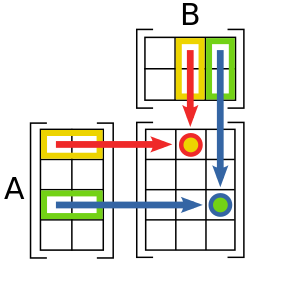
\includegraphics[width=\marginparwidth]{figures/matrixmul.png}
	\caption{矩阵乘法}\label{matrixmul}
\end{marginfigure}

自然而然,我们会想,矩阵是否有乘法运算.我们可以给矩阵的乘法运算进行以下定义:
\begin{definition}[\textbf{矩阵乘法}]
	设矩阵$\mathbf{A}=\left(a_{ij}\right)_{m\times s},\mathbf{B}=\left(b_{ij}\right)_{s\times n}$,规定$\mathbf{A}$与$\mathbf{B}$的乘积为矩阵$\mathbf{C}=\left(c_{ij}\right)_{m\times n},$记为$\mathbf{AB=C}$,其中
	\[
		c_{ij}=a_{i1}b_{1j}+a_{i2}b_{2j}+\cdots+a_{is}b_{sj}=\sum_{k=1}^{s}a_{ik}b_{kj},i=1,2,\cdots ,m;j=1,2,\cdots ,n.
	\]
\end{definition}

也就是说:$\mathbf{AB}$的$\left(i,j\right)$元素为$\mathbf{A}$的第$i$行各元素分别与$\mathbf{B}$的第$j$列对应元素的乘积之和.

注意:\textbf{如果$\mathbf{AB}$可以相乘,那么$\mathbf{A}$的列数一定等于$\mathbf{B}$的行数.}

左图\ref{matrixmul}可以帮助理解矩阵的乘法.

根据矩阵乘法的定义,我们可以将旋转变换\eqref{tran1}式写做:
\[
	\begin{bmatrix}
		x \\
		y
	\end{bmatrix}
	=\begin{bmatrix}
		\cos\theta & -\sin\theta \\
		\sin\theta & \cos\theta
	\end{bmatrix}
	=\begin{bmatrix}
		x' \\
		y'
	\end{bmatrix}.
\]
这里,我们也可以看出这样定义矩阵乘法的合理性.

\begin{example}
	设矩阵\[
		\mathbf{A}=
		\begin{bmatrix}
			a_{1}  \\
			a_{2}  \\
			\vdots \\
			a_{n}
		\end{bmatrix}  ,
		\mathbf{B}=
		\begin{bmatrix}
			b_{1} & b_{2} & \cdots & b_{n}
		\end{bmatrix}  ,
	\]
	求$\mathbf{AB}$与$\mathbf{BA}$.
\end{example}
\begin{solution}
	\[
		\mathbf{AB}=\begin{bmatrix}
			a_{1}  \\
			a_{2}  \\
			\vdots \\
			a_{n}
		\end{bmatrix}
		\begin{bmatrix}
			b_{1} & b_{2} & \cdots & b_{n}
		\end{bmatrix}
		=\begin{bmatrix}
			a_{1}b_1 & a_{1}b_2 & \cdots & a_{1}b_n \\
			a_{2}b_1 & a_{2}b_2 & \cdots & a_{2}b_n \\
			\vdots   & \vdots   & \ddots & \vdots   \\
			a_{n}b_1 & a_{n}b_2 & \cdots & a_{n}b_n
		\end{bmatrix}  ,
	\]\[
		\mathbf{BA}=\begin{bmatrix}
			b_{1} & b_{2} & \cdots & b_{n}
		\end{bmatrix}
		\begin{bmatrix}
			a_{1}  \\
			a_{2}  \\
			\vdots \\
			a_{n}
		\end{bmatrix}
		=b_1a_1+b_2a_2+\cdots +b_na_n.
	\]
\end{solution}

可以看出,在矩阵乘法中,$\mathbf{AB}$不一定等于$\mathbf{BA}$.也就是说,\textbf{矩阵的乘法运算不满足交换律}.

矩阵乘法满足以下运算规律:
\begin{enumerate}
	\item 有单位元:$\mathbf{I}_m \mathbf{A}_{m\times n}=\mathbf{A}_{m\times n}\mathbf{I}_n=\mathbf{A}_{m\times n}$;
	\item 乘法结合律:$\mathbf{(AB)C=A(BC)}$;
	\item 数乘的结合律:$(k\mathbf{A})\mathbf{B}=\mathbf{A}(k\mathbf{B})=k\mathbf{(AB)}$;
	\item 左分配律:$\mathbf{A(B+C)=AB+BC}$;
	\item 右分配律:$\mathbf{(A+B)C=AC+BC}$.
\end{enumerate}

在这节课的开始,我们介绍了关于旋转变换的例子,我们看到一个旋转变换和一个矩阵一一对应.事实上,用矩阵来表示此类的变换,是矩阵最重要的作用之一.下面我们将介绍线性变换与矩阵的关系.

设有变量$x_1,x_2,\cdots,x_n$到变量$y_1,y_2,\cdots,y_m$的变换
\begin{equation}
	\label{le}
	\left\{\begin{matrix}
		y_1=a_{11}x_1+a_{12}x_2+\cdots+a_{1n}x_n, \\
		y_2=a_{21}x_1+a_{22}x_2+\cdots+a_{2n}x_n, \\
		\cdots\cdots\cdots\cdots                  \\
		y_m=a_{m1}x_1+a_{m2}x_2+\cdots+a_{mn}x_n,
	\end{matrix}\right.
\end{equation}
这个线性方程组也可以写成矩阵形式:
\[
	\begin{bmatrix}
		y_{1}  \\
		y_{2}  \\
		\vdots \\
		y_{m}
	\end{bmatrix}
	=\begin{bmatrix}
		a_{11} & a_{12} & \cdots & a_{1n} \\
		a_{21} & a_{22} & \cdots & a_{2n} \\
		\vdots & \vdots & \ddots & \vdots \\
		a_{m1} & a_{m2} & \cdots & a_{mn}
	\end{bmatrix}
	\begin{bmatrix}
		x_{1}  \\
		x_{2}  \\
		\vdots \\
		x_{n}
	\end{bmatrix},
\]
或
\begin{equation}
	\label{le2}
	\mathbf{y=Ax},
\end{equation}
其中,$\mathbf{A}=\left(a_{ij}\right)_{m\times n},
	\mathbf{x}=	\begin{bmatrix}
		x_{1}  \\
		x_{2}  \\
		\vdots \\
		x_{n}
	\end{bmatrix},
	\mathbf{y}=	\begin{bmatrix}
		y_{1}  \\
		y_{2}  \\
		\vdots \\
		y_{m}
	\end{bmatrix}.$

我们称\eqref{le}式或\eqref{le2}是一个由$n$维向量到$m$维向量的\textbf{线性变换}.显然,这个线性变换由矩阵$\mathbf{A}$完全确定,我们称$\mathbf{A}$为线性变换\eqref{le}的矩阵.

现在,我们需要明确,\textbf{每一个线性变换都完全由一个矩阵确定},在一些问题中,我们完全可以把线性变换用矩阵替换,把矩阵用线性变换替换.

下面将介绍几个线性变换的例子.
\begin{example}[\textbf{反射变换}]
	在平面直角坐标系$Oxy$内任意一点$P$变成关于$x$轴的对称点,该线性变换对应的矩阵为
	$\begin{bmatrix}
			1 & 0  \\
			0 & -1
		\end{bmatrix} $.
\end{example}
\begin{example}[\textbf{伸缩变换}]
	在平面直角坐标系$Oxy$内任意一点$P$的纵坐标变为原来的$k$倍,该线性变换对应的矩阵为
	$\begin{bmatrix}
			1 & 0 \\
			0 & k
		\end{bmatrix} $.
\end{example}
\begin{example}[\textbf{投影变换}]
	在平面直角坐标系$Oxy$内任意一点$P$在$x$轴上的投影变换,该线性变换对应的矩阵为
	$\begin{bmatrix}
			1 & 0 \\
			0 & 0
		\end{bmatrix} $.
\end{example}

我们已经给出一个线性变换\eqref{le2},同样的,一个$p\times m$矩阵$B$也可以确定一个线性变换:
\begin{equation}
	\label{le3}
	\mathbf{z=By},
\end{equation}

现在,我们要求线性变换\eqref{le2}和线性变换\eqref{le3}的复合变换,即
\begin{equation}
	\label{le4}
	\mathbf{z=By=B(Ax)=(BA)x}.
\end{equation}

可见,线性变换\eqref{le4}的矩阵为$\mathbf{BA}$.

在这里我们可以看出,用矩阵处理线性变换的便利之处.同时,矩阵也可以用来处理线性方程组:

对于线性方程组
\begin{equation}
	\label{eq}
	\left\{\begin{matrix}
		a_{11}x_1+a_{12}x_2+\cdots+a_{1n}x_n=b_1, \\
		a_{21}x_1+a_{22}x_2+\cdots+a_{2n}x_n=b_2, \\
		\cdots\cdots\cdots\cdots                  \\
		a_{m1}x_1+a_{m2}x_2+\cdots+a_{mn}x_n=b_m,
	\end{matrix}\right.
\end{equation}

我们可以将其写成矩阵形式
\[
	\begin{bmatrix}
		a_{11} & a_{12} & \cdots & a_{1n} \\
		a_{21} & a_{22} & \cdots & a_{2n} \\
		\vdots & \vdots & \ddots & \vdots \\
		a_{m1} & a_{m2} & \cdots & a_{mn}
	\end{bmatrix}
	\begin{bmatrix}
		x_{1}  \\
		x_{2}  \\
		\vdots \\
		x_{n}
	\end{bmatrix}
	=\begin{bmatrix}
		b_{1}  \\
		b_{2}  \\
		\vdots \\
		b_{m}
	\end{bmatrix}
\]

或
\begin{equation}
	\mathbf{Ax=b},
\end{equation}

我们称$\mathbf{A}$为方程组\eqref{eq}的\textbf{系数矩阵},在系数矩阵$\mathbf{A}$的右侧再加一列列向量$\mathbf{b}$,则可组成$m\times(n+1)$矩阵
\[
	\overline{\mathbf{A}}=
	\begin{bmatrix}
		a_{11} & a_{12} & \cdots & a_{1n} & b_1    \\
		a_{21} & a_{22} & \cdots & a_{2n} & b_2    \\
		\vdots & \vdots & \ddots & \vdots & \vdots \\
		a_{m1} & a_{m2} & \cdots & a_{mn} & b_m
	\end{bmatrix} ,
\]

称$\overline{\mathbf{A}}$为方程组\eqref{eq}的\textbf{增广矩阵}.显然,线性方程组的增广矩阵完全确定了这个线性方程组.

如果$x_1=c_1,x_2=c_2,\cdots,x_n=c_n$是方程组\eqref{eq}的一个解,则
\[
	x_0=\begin{bmatrix}
		c_{1}  \\
		c_{2}  \\
		\vdots \\
		c_{n}
	\end{bmatrix}
\]
称为线性方程组\eqref{eq}的\textbf{解向量}.

最后,我们再来定理方阵的幂.
对于$n$阶方阵$A$,考虑到矩阵满足乘法结合律,我们可以定义$A$的幂为
\[
	\mathbf{A}^0=I,\mathbf{A}^m=\underset{m\text{个}}{\mathbf{A}\mathbf{A}\cdots \mathbf{A}}.\]
显然也有:
\[
	\mathbf{A}^k\mathbf{A}^l=\mathbf{A}^{kl},(\mathbf{A}^k)^l=\mathbf{A}^{kl}.
\]

\section{矩阵的转置}
\begin{definition}[\textbf{矩阵转置}]
	把$m\times n$矩阵$\mathbf{A}$的行依次换成列(列依次换成行)所得到的$n\times m$矩阵,称为$\mathbf{A}$的转置矩阵,记为$\mathbf{A}^T$.
\end{definition}

\begin{example}
	$\mathbf{A}=\begin{bmatrix}
			-2 & 3 \\
			0  & 7 \\
			6  & 5
		\end{bmatrix}$
	的转置矩阵$\mathbf{A}^T=
		\begin{bmatrix}
			-2 & 0 & 6 \\
			3  & 7 & 5
		\end{bmatrix}.$
\end{example}

矩阵的转置满足以下运算规律:
\begin{enumerate}
	\item $(\mathbf{A}^T)^T=A$;
	\item $\mathbf{(A+B)}^T=\mathbf{A}^T+\mathbf{B}^T;$
	\item $(k\mathbf{A})^T=k\mathbf{A}^T;$
	\item $(\mathbf{AB})^T=\mathbf{B}^T\mathbf{A}^T.$
\end{enumerate}
第四条规律较为特殊,请同学们牢记.第四条规律也可以推广:
\[
	(\mathbf{A}_1\mathbf{A}_2\cdots \mathbf{A}_m)^T=\mathbf{A}_{m}^{T}\cdots \mathbf{A}_{2}^{T}\mathbf{A}_{1}^{T}.
\]

下面再介绍两个特殊矩阵.
\begin{definition}[\textbf{对称矩阵}]
	若方阵$\mathbf{A}=(a_{ij})_{n\times n}$满足$\mathbf{A}^T=\mathbf{A}$,则称$\mathbf{A}$为\textbf{对称矩阵}.
\end{definition}

\begin{definition}[\textbf{反对称矩阵}]
	若方阵$\mathbf{A}=(a_{ij})_{n\times n}$满足$\mathbf{A}^T=-\mathbf{A}$,则称$\mathbf{A}$为\textbf{反对称矩阵}.
\end{definition}
$\star$注意对称矩阵和反对称矩阵都是方阵.

\section{方阵的行列式}
我们已经在第一章了解过行列式,至此,我们也发现行列式与矩阵在形式上有很多相似之处.下面我们来介绍方阵的行列式.

\begin{definition}
	对于$n$阶方阵$\mathbf{A}=(a_{ij})_{n\times n}$,称$n$阶行列式
	\[
		\begin{vmatrix}
			a_{11} & a_{12} & \cdots & a_{1n} \\
			a_{21} & a_{22} & \cdots & a_{2n} \\
			\vdots & \vdots & \ddots & \vdots \\
			a_{n1} & a_{n2} & \cdots & a_{nn}
		\end{vmatrix}
	\]
	为方阵$\mathbf{A}$的行列式,记为$\det(\mathbf{A})$.
\end{definition}

方阵的行列式满足以下运算规律:
\begin{enumerate}
	\item $\det(\mathbf{A}^T)=\det(\mathbf{A})$;
	\item $\det(k\mathbf{A})=k^n \det(\mathbf{A})$;
	\item $\det(\mathbf{AB})=\det(\mathbf{A})\cdot \det(\mathbf{B})$.
\end{enumerate}
第三条规律也可以推广:
\[
	\det(\mathbf{A}_1\mathbf{A}_2\cdots \mathbf{A}_m)=\det(\mathbf{A}_1)\det(\mathbf{A}_2)\cdots\det(\mathbf{A}_m).
\]